%%%%%%%%%%%%%%%%%%%%%%%%%%%%%%%%%%%%%%%%%%%%%%%%%%%%%%%%%%%%%%%%%%%%%%%%%%%%
% AGUtmpl.tex: this template file is for articles formatted with LaTeX2e,
% Modified March 2013
%
% This template includes commands and instructions
% given in the order necessary to produce a final output that will
% satisfy AGU requirements.
%
% PLEASE DO NOT USE YOUR OWN MACROS
% DO NOT USE \newcommand, \renewcommand, or \def.
%
% FOR FIGURES, DO NOT USE \psfrag or \subfigure.
%
%%%%%%%%%%%%%%%%%%%%%%%%%%%%%%%%%%%%%%%%%%%%%%%%%%%%%%%%%%%%%%%%%%%%%%%%%%%%
%
% All questions should be e-mailed to latex@agu.org.
%
%%%%%%%%%%%%%%%%%%%%%%%%%%%%%%%%%%%%%%%%%%%%%%%%%%%%%%%%%%%%%%%%%%%%%%%%%%%%
%
% Step 1: Set the \documentclass
%
% There are two options for article format: two column (default)
% and draft.
%
% PLEASE USE THE DRAFT OPTION TO SUBMIT YOUR PAPERS.
% The draft option produces double spaced output.
%
% Choose the journal abbreviation for the journal you are
% submitting to:

% jgrga JOURNAL OF GEOPHYSICAL RESEARCH
% gbc   GLOBAL BIOCHEMICAL CYCLES
% grl   GEOPHYSICAL RESEARCH LETTERS
% pal   PALEOCEANOGRAPHY
% ras   RADIO SCIENCE
% rog   REVIEWS OF GEOPHYSICS
% tec   TECTONICS
% wrr   WATER RESOURCES RESEARCH
% gc    GEOCHEMISTRY, GEOPHYSICS, GEOSYSTEMS
% sw    SPACE WEATHER
% ms    JAMES
% ef    EARTH'S FUTURE
%
%
%
% (If you are submitting to a journal other than jgrga,
% substitute the initials of the journal for "jgrga" below.)

\documentclass[draft,grl]{AGUTeX}
% To create numbered lines:

% If you don't already have lineno.sty, you can download it from
% http://www.ctan.org/tex-archive/macros/latex/contrib/ednotes/
% (or search the internet for lineno.sty ctan), available at TeX Archive Network (CTAN).
% Take care that you always use the latest version.

% To activate the commands, uncomment \usepackage{lineno}
% and \linenumbers*[1]command, below:

\usepackage{lineno}
\usepackage{amssymb}
\usepackage{amsmath}
\usepackage{textcomp}
\usepackage[super]{nth}
\usepackage{tabularx}
\usepackage{multirow}
\usepackage{bm}
\usepackage{color} 
\usepackage{hyperref}

\linenumbers*[1]

%  To add line numbers to lines with equations:
%  \begin{linenomath*}
%  \begin{equation}
%  \end{equation}
%  \end{linenomath*}
%%%%%%%%%%%%%%%%%%%%%%%%%%%%%%%%%%%%%%%%%%%%%%%%%%%%%%%%%%%%%%%%%%%%%%%%%
% Figures and Tables
%
%
% DO NOT USE \psfrag or \subfigure commands.
%
%  Figures and tables should be placed AT THE END OF THE ARTICLE,
%  after the references.
%
%  Uncomment the following command to include .eps files
%  (comment out this line for draft format):
\usepackage[final]{graphicx}
%
%  Uncomment the following command to allow illustrations to print
%   when using Draft:
%  \setkeys{Gin}{draft=false}
%
% Substitute one of the following for [dvips] above
% if you are using a different driver program and want to
% proof your illustrations on your machine:
%
% [xdvi], [dvipdf], [dvipsone], [dviwindo], [emtex], [dviwin],
% [pctexps],  [pctexwin],  [pctexhp],  [pctex32], [truetex], [tcidvi],
% [oztex], [textures]
%
% See how to enter figures and tables at the end of the article, after
% references.
%
%% ------------------------------------------------------------------------ %%
%
%  ENTER PREAMBLE
%
%% ------------------------------------------------------------------------ %%

% Author names in capital letters:
\authorrunninghead{DAY ET AL.}

% Shorter version of title entered in capital letters:
\titlerunninghead{THE ``SOUTH FLOOD-NORTH DROUGHT'' IN MEIYU AND JET STATS}

%Corresponding author mailing address and e-mail address:
\authoraddr{Corresponding author: Jesse Day, University of California Berkeley, Department of Earth and Planetary Science, College of Letters and Science; 307 McCone Hall, Berkeley, CA 94720, USA. (jessed@berkeley.edu)}

\begin{document}

%% ------------------------------------------------------------------------ %%
%
%  TITLE
%
%% ------------------------------------------------------------------------ %%


\title{Signature of the ``South Flood-North Drought" in Meiyu Front and Tropospheric Jet Changes}

%% ------------------------------------------------------------------------ %%
%
%  AUTHORS AND AFFILIATIONS
%
%% ------------------------------------------------------------------------ %%


%Use \author{\altaffilmark{}} and \altaffiltext{}

% \altaffilmark will produce footnote;
% matching \altaffiltext will appear at bottom of page.

\authors{Jesse A. Day\altaffilmark{1},
Jacob P. Edman\altaffilmark{1}, John C. H. Chiang\altaffilmark{2}, Inez Fung \altaffilmark{1}, and
Weihan Liu\altaffilmark{3}}

\altaffiltext{1}{Department of Earth and Planetary Science, University of California Berkeley, Berkeley, California, USA.}
\altaffiltext{2}{Department of Geography, University of California Berkeley, Berkeley, California, USA.}
\altaffiltext{3}{College of Letters and Science, University of California Berkeley, Berkeley, California, USA.}


%% ------------------------------------------------------------------------ %%
%
%  ABSTRACT
%
%% ------------------------------------------------------------------------ %%

% >> Do NOT include any \begin...\end commands within
% >> the body of the abstract.

%Needs to be 150 words or less - currently at 132.
\begin{abstract}
We have created a novel 57-year (1951-2007) daily catalog of frontal rainbands over China from APHRODITE rain gauge data, and present an unprecedented climatology of Meiyu front progression in summer. We investigate late \nth{20} century changes in Chinese summer rainfall (the ``South Flood-North Drought''). Two robust changes in front behavior are observed during 1980-2007 relative to 1951-1979: 1) A significant decrease in the frequency of Pre-Meiyu (May) frontal rainbands, and 2) a southward shift in the latitude of Post-Meiyu rainbands (mid-July to September). In addition, the mean latitude of the tropospheric jet has shifted southward during both time periods. We propose that both frontal changes reflect an overall southward displacement of the tropospheric jet's cycle during summer. Our results hold the potential of coupling regional climate change to \nth{21} century global change. 

\end{abstract}

%% Allowed length of manuscript is (# of words/500) + # of figures + # of tables.

%currently: 3509 words + 5 figures (max words: 3500)

\begin{article}

\section{Introduction}
 
 	China receives about 60\% of its rainfall from May to August, a period known collectively as the East Asian summer monsoon. The period of peak rainfall within this monsoon lasts from early June to mid-July (usually referred to as ``Meiyu Season'') and features a northward-migrating front known as the Meiyu front (lit. ``Plum rains,'' referring to the spectacular growth of plum blossoms in central China coincident with the onset of heavy rains). The corresponding rainy seasons in Japan and Korea are known as Baiu and Changma respectively. A growing volume of evidence suggests a shift in mean rainfall patterns over China beginning in the late 1970s, with increased flooding in the south and droughts in the north (the ``South Flood-North Drought'') \citep{Hu1997,Gong2002,Nigam2013}. The yearly mean change in rainfall rate is shown in Figure \ref{changes_2d}. A permanent change would have major humanitarian impacts on densely-populated eastern China, where a sizable fraction of the population depends on agriculture for subsistence. Northern China already suffers from substantial depletion of freshwater resources along with increasing demand \citep{Currell2012,Gleeson2012}. The Chinese government has already embarked on a project to reroute water from the Yangtze River to northern China, the South-North Water Transfer Project (\textit{nanshui beidiao gongcheng}), which is expected to become the most expensive hydraulic engineering project ever undertaken and will entail massive human and environmental impact \citep{Magee2011}.
 
	Although summer rainfall in East Asia is referred to as a monsoon, its climatology bears little resemblance to its Indian counterpart or other monsoon circulations worldwide \citep{Ding2005}. Whereas understanding of tropical monsoons has progressed greatly via theoretical studies \citep{Plumb1992,Prive2007,Bordoni2008}, the dynamics that favor the existence of frontal convection over East Asia in summer remain a point of debate, centering around the interplay of the tropospheric jet and Tibetan Plateau \citep{Molnar2010,Sampe2010,Chen2014}. Therefore, no simple conceptual template exists for interpreting a change such as the South Flood-North Drought. However, it is known that the migration of the Meiyu front entails a series of large-scale circulation changes \citep{Chen2004}, and furthermore that anomalies in Meiyu front latitude produce corresponding rainfall anomalies \citep{Kosaka2011}. Therefore, a long-term change in rainfall r\'egime such as the South Flood-North Drought should be describable in terms of changes in the characteristics of Meiyu rainbands, such as a shift in latitude, a change in intensity or an earlier or later transition from one stage to the next. In turn, such a characterization may provide insight into the dynamics responsible for the change.
	
	In pursuit of this aim, we have developed a 57-year climatology (1951-2007) of frontal rainbands in China based on the APHRODITE rain gauge product (described below). We develop a convergent fitting algorithm of daily rainfall maps which determines whether a front exists, and if so, measures its attributes. A few previous studies have discussed the statistics of the Meiyu front on decadal and even centennial time scales \citep{Chen2004,Ge2008,Xu2009}, but to our knowledge no author has compiled a multi-decadal daily catalog of events. We use this database to clarify the spatial and temporal characteristics of the South Flood-North Drought, and present it as a tool for future East Asian monsoon research.
		
	We also explore links between the behavior of the Meiyu front and subtropical jet, which plays an essential and complex role in East Asian climate both in summer and winter \citep{Yang2002}. In a region featuring a strong wind shear, we expect a band of ascent displaced southward from the core of maximum wind \citep{Holton2004}. Theoretical studies suggest that the high topography of the Tibetan Plateau couples with the jet in nonlinear fashion, amplifying the regional response to global climate anomalies \citep{Nigam1989,Broccoli1992,Park1997}. In summer, past work has argued the timing of the jet's transit north of the Tibetan Plateau dictates the initiation of the monsoon in India and East Asia, both in present-day \citep{Yin1949,Yeh1959,Hahn1975} and on paleoclimate timescales \citep{Nagashima2011,Nagashima2013,Chiang2015}. Meridional shifts in the tropospheric jet induce rainfall anomalies in China \citep{Liang1998}, as do changes in its strength \citep{Kwon2007,Du2009,Li2014} On a daily time scale, the jet serves as a waveguide for storms propagating from the Euarasian interior via the ``Silk Road'' teleconnection \citep{Hoskins1993,Ambrizzi1997,Kosaka2012}. Thus, it is reasonable to expect \nth{20} century changes in the tropospheric jet over East Asia in conjunction with Meiyu changes. Therefore, we compare our Meiyu database with an existing data set of jet counts for 1958-2001, as described in \citet{Schiemann2009}, in search of coupled change.
	
\section{Data and Methods}

\subsection{APHRODITE Rainfall Data}

	The APHRO\_MA\_V1101 product from APHRODITE (Asian Precipitation - Highly-Resolved Observational Data Integration Towards Evaluation of the Water Resources) includes 57 years (1951-2007) of daily  rainfall derived from rain gauge records (and therefore available over land only) \citep{Yatagai2012} . Available data are precipitation (PRECIP product, units mm day$^{-1}$) and station coverage (RSTN product) on a .25\textdegree\ $\times$ .25\textdegree\ grid (roughly 25 km spacing) between 60\textdegree E-150\textdegree E and 15\textdegree S-55\textdegree N. We focus on the subregion of land lying within 100\textdegree E-123\textdegree E and 20\textdegree N-40\textdegree N as the area of occurrence of Meiyu rainbands. Station observations in eastern China are spaced at roughly 100 to 200 km intervals sufficient to resolve frontal events. APHRODITE's resolution cannot represent some features visible in TRMM satellite data, such as the anchoring of rainfall by low orography \citep{Xu2009}. In compensation, the length of our data set allows us to study decadal change in frontal properties. 
	
\subsection{A Database of Jet Counts from \citet{Schiemann2009}} 

	\citet{Schiemann2009} constructed a data set of jet `counts' in the Tibetan Plateau region (46\textdegree E-130\textdegree E, 17\textdegree N-58\textdegree N) from ERA-40 reanalysis for 1958-2001, where a count is defined as any local maximum in the horizontal wind field with westerly magnitude greater than $30$ m s$^{-1}$; further details can be found in section 2 of \citet{Schiemann2009}. We focus on the longitude subset of $90-130^\circ$E, which encompasses the region of Meiyu front activity, and present jet latitude averaged across this longitude range in Figure \ref{jet_seasonal}. Our results are not sensitive to the exact choice of longitude range. In addition, Figure 2 presents contours of jet frequency estimated by a kernel density method, which estimates probability distribution from a set of discrete data observations. We obtain binned kernel density estimates using a standard bivariate normal kernel. 
	
\subsection{Front Detection Algorithm}

	For each day from 1 January 1951 to 31 December 2007 (20,819 days total), a convergent recursive image processing algorithm determines whether a frontal rainfall rainband exists inside the window of 105-123E and 20-40N. On a given day, rainfall over China must include a continuous chain of rainfall maxima over 5 degrees exceeding 10 mm day$^{-1}$. If one exists, we perform a recursive weighted linear fit and measure properties of the rainband including the latitude, mean intensity, tilt, length and width, as well as the ``quality score'' $Q$ - what percentage of daily rainfall in China falls within our calculated band. Days that do not meet a minimum $Q$ value of .6 are treated as days without fronts. We also test for the possibility of two frontal events occurring on a single day, an arrangement commonly seen in August and September. Subsequently, we use the terminology of ``primary'' and ``secondary'' front for such days. We also test for false positives dominated by heavy local rainfall over Taiwan. The full workings of the algorithm are listed in the supplementary material, along with statistics of its output and examples of its functionality.
	
	%note - transfer relevant citations to supplemental cites.

\subsection{Statistical Significance of Changes in Means}

	Two separate Monte Carlo methods are employed to assess the statistical significance of the change in mean between time periods: 1) Bootstrapping with replacement and 2) a permutation test (without replacement) \citep{Good2005}. Calculations of significance are executed by performing 10,000 iterations of each algorithm and comparing actual values to the synthetic distributions. In the text that follows we have presented the results of the permutation test, which are extremely similar to the results of bootstrapping with replacement, but generally stricter. Both algorithms are further discussed in supplementary material. In calculating the significance of changes in frontal behavior in 1980-2007 relative to 1951-1979, we have repeated all calculations of significance for the years 1980-2001 versus 1958-1979, which are the years when jet count data is available. The results remain the same unless otherwise noted.

%MOVING BLOCKS BOOTSTRAP - must test use
%Provide code of bootstrapping algorithms in supplementary information?

\section{Frontal Behavior}	
	
\subsection{Climatology}	

	The yearly progression of precipitation over eastern China is shown in Figure \ref{hov}a, averaged over $100^\circ-123^\circ$E with a 5-day running mean, similar to Figure 7 in \citet{Ding2005}. China receives a substantial fraction of its yearly precipitation outside of summer, unlike a traditional monsoonal region. Figure \ref{hov}b shows a Hovm\"oller diagram of the frequency of frontal rainfall over all 57 years, including both primary and secondary rainbands. It can be seen that some periods of heavy rainfall, in particular the August peak over southern China (over 10 mm day$^{-1}$ around 20\textdegree N), do not correspond to a surge in frontal events. Figure \ref{hov}c shows the probability of observing a front and its mean intensity, and Figure \ref{hov}d shows other ancillary characteristic including the frequency of a secondary front, mean tilt and mean length. Frontal rainbands over China can occur in any month, with their intensity and probability of occurrence minimizing in January (12 mm day$^{-1}$ and 10\% probability occurrence) and maximizing in late June (31 mm day$^{-1}$ and 80\% probability of occurrence).
	
	Figures \ref{hov}a-d show coordinated sharp changes in rainfall and frontal properties. We define 5 periods of notable frontal behavior as demarcated in Figure \ref{hov}: 1) The ``Spring Rains'' for days 60-120 (March 1-April 30), as previously studied in \citet{Tian1998}; 2) The ``Pre-Meiyu,'' days 121-160 (May 1-June 9), when rainfall and front intensity increase; 3) Meiyu season from days 161 to 200, when frontal frequency and intensity peaks and a remarkable 7-degree northward shift in preferred latitude occurs (June 10-July 19); 4) The Post-Meiyu from days 201-273, during which double fronts are common (July 20-September 30) and 5) the ``Fall Rains,'' days 274-320 (October 1-November 16), during which the front returns south. The mean and standard deviation of frontal properties during each time period is presented in Supplementary Table S1. In addition, Figures \ref{climo}a-e shows mean rainfall, jet frequency and front position during each of these stages. The Pre-Meiyu, Meiyu and Post-Meiyu are equivalent to the three stages of Meiyu rainfall described in \citet{Ding2005}. Our results can be compared with the event catalog of \citet{Xu2009}, which finds a similar date for the northward transition of the Meiyu front. We note that there are more frequent and intense Meiyu rainbands in spring than in fall, and that the northward transit of the front (Meiyu season) induces much more rainfall than its southward return (the Fall Rains). The dynamical cause of this yearly asymmetry deserves further study.
		
\subsection{Front Changes, 1980-2007 Versus 1951-1979}
	
	We calculate changes in rainfall and frontal frequency in 1980-2007 versus 1951-1979 and their statistical significance. The results are shown in Figure \ref{changes} and Supplementary Table S2. In addition, Figures \ref{changes_2d}f-g show spatial changes in rainfall and front behavior during the Pre- and Post-Meiyu, when changes are particularly large. The greatest change in frontal behavior has occurred during Pre-Meiyu season (days 121-160, or May 1-June 9), when the probability of observing a frontal event has declined from $60.7\% \pm 1.5\%$ to $52.2\% \pm 1.6\%$ (statistical significance of $p < .0002$). A corresponding decrease in Pre-Meiyu rainfall has occurred in central China (Figure 2f and 30\textdegree N in Figure \ref{changes}a). The change in Pre-Meiyu rainfall in the late \nth{20} century has previously been reported by \citet{Xin2006} and \citet{Wang2009}.
		
	In addition, a southward shift in mean frontal latitude has occurred during the Post-Meiyu (days 201-273, or July 20-Sep 30). Mean latitude from 1951-1979 was $29.9^\circ \textrm{N} \pm .3^\circ$ versus $29.3^\circ \textrm{N} \pm .4^\circ$, a difference significant at a 95\% confidence level. During the same time period, a rainfall increase in central China and decrease in northern China has occurred (Figure 2g and Figure \ref{changes}a), whose spatial distribution resembles the template of the ``South Flood-North Drought.'' As a result, yearly rainfall has increased in central China even though Pre-Meiyu rainfall changes in that region are negative. Unlike \citet{Yu2010},  our catalog does not exhibit a decrease in the intensity of Yangtze River region frontal rainbands during July-August. A statistically significant southward shift in front latitude is also found for the whole year (Table S2), but the signal is dominated by the change in Post-Meiyu frontal behavior.
	
\section{Jet}

\subsection{Dynamics}

	The interaction of the tropospheric jet with the Tibetan Plateau is crucial to producing convergence and frontal rainfall downstream over China and the western Pacific Ocean \citep{Molnar2010,Sampe2010,Chen2014}. Peak rainfall rates in China from May to mid-July corresponds to the months when the climatological latitude of the jet impinges on the Tibetan Plateau \citep{Schiemann2009}. The tropospheric jet marks the northern boundary of the Hadley Cell, and shifts in response to seasonal changes in insolation. In summer, the East Asian tropospheric jet shifts from its winter position on the southern flank of the Tibetan Plateau to a summer latitude well north of the plateau. During the transition, the jet occupies intermediate configurations that correspond to different stages of China rainfall (Figure \ref{climo}). A full monthly climatology of the jet is visible in \citet{Schiemann2009}. From May to September,  the climatological latitudes of rainfall, fronts and the jet are closely coupled, with the jet shifted about 5-10 degrees north of the latitude of peak rainfall. The initiation of the Pre-Meiyu corresponds roughly to the beginning of the jet's northward passage. During Meiyu season, the preferred latitude of the jet continues to transition northward. The period of frequent double front occurrence during the Post-Meiyu corresponds to the jet's maximal northward extent. Finally, the ``Fall rains'' in October and November correspond to the shift of the jet back southward of the Tibetan Plateau, with a weak rainfall response.
	
\subsection{Jet Changes, 1980-2001 Versus 1958-1979}

	In Figure \ref{jet_seasonal}a, we show the mean jet latitude from April to October in the region $90-130^\circ$E, averaged over the years 1958-1979 (blue solid line) and 1980-2001 (dashed red line). The significant changes in front behavior described in the previous section both correspond to southward shifts in mean jet latitude. During the Pre-Meiyu (May), the tropospheric jet is shifted southward by almost 2\textdegree\ in 1980-2001 relative to 1958-1979, when its mean latitude was $\approx 41^\circ$N. {\color{blue} We estimate the significance of this change using a two-tailed Kolmogorov-Smirnov (K-S) test, and find a $p=0.003998$. Since the K-S test assumes all samples are independent, we remove autocorrelation due to synoptic variability by considering the mean jet latitude over 4 day periods, rather than the daily mean. To see that this procedure removes the autocorrelation, see the supplement.} During the Post-Meiyu (days 201-273), when the mean latitude of Meiyu rainbands has shifted south during 1980-2007, the mean latitude of the jet is consistently southward during 1980-2001 relative to 1958-1979. {\color{blue} Similar to the procedure for the pre-Meiyu period, we perform a K-S test on the 7-day mean jet latitude, and find the $p=0.05667$.  }
	
%provide some kind of measure of the probability value of the entire shift?
	
\section{Hypothesis}

{\color{red}  I propose changing the title of this section to `discussion' and reorganizing this and the conclusion section. I'll add my suggested additions to the this section in blue }  

	Given the covariance of Meiyu front and tropospheric jet latitude in the climatological mean and the joint changes in fronts and jet counts between 1951-1979 and 1980-2007 , the ``South Flood-North Drought'' appears to reflect an alteration in jet dynamics. We propose that both the Pre-Meiyu decline in front frequency and the Post-Meiyu southward shift reflect a single phenomenon: the southward displacement of the jet's seasonal progression. In climatology, the Pre-Meiyu corresponds to the beginning of the jet's transit, when it first impinges on the Tibetan Plateau. If the latitude cycle of the jet is shifted southward, the jet will impinge on the Tibetan Plateau later, delaying the onset of the Pre-Meiyu. Instead, we would expect prolonged Spring Rain conditions, when central China rainfall is weaker and front frequency is lower. Furthermore, the southward shift of the jet during the post-Meiyu has shifted the latitude of frontal events southward during that period. Thus, our hypothesis can explain both the Pre-Meiyu and Post-Meiyu changes in front behavior and rainfall. In the annual mean, the net effect of the southward jet shift would be a rainfall decrease in northern China and an increase in central China, producing a ``South Flood-North Drought'' response.
	
	In support of our hypothesis, Figure \ref{jet_seasonal}b shows a scatter plot of May (Days 121-150) front frequency anomalies versus tropospheric jet anomalies. Most years with a decrease in front frequency feature a southward jet shift, and vice-versa. During the Post-Meiyu, a similar relation is found between monthly anomalies in front latitude and jet latitude (Figure \ref{jet_seasonal}c). In this case, we remove frontal events south of 28\textdegree N, since they arrive from the South China Sea \citep{Day2015} and are therefore not directly related to the jet.

{\color{blue} 
	 Observations show that the global annual mean latitude of the tropospheric jet has shifted poleward, in tandem with mid-latitude tropospheric heating, increased subtropical static stability, a northward shift in mean ITCZ latitude and the expansion of the Hadley circulation \citep{Fu2006,Archer2008,Fu2011}. Opposite trends are found in some regions and the variation by season is significant;  we find that the East Asian portion of the jet has shifted equatorward, in agreement with past studies \citep{Yu2007, Archer2008}. Recent work suggests that the southward displacement of the jet over the Pacific Ocean has resulted from late \nth{20} century changes in tropical Pacific convection and SST \citep{Park2014a}. Thus, the global poleward trend in jet latitude and the East Asian equatorward shift are compatible observations that result from the heterogeneous spatial distribution of \nth{20} century warming.
	 
	 In addition to the change in China rainfall in the late 1970s, authors have reported an earlier onset of the Pre-Meiyu season over the period 1994-2008 relative to 1979-1993 \citep{Kajikawa2012}, as well as an increase in rainfall over southeastern China and in the passage of tropical cyclones \citep{Kwon2007,Chang2014}. We repeat the analysis of Section 4 for the two time periods 1979-1993 and 1994-2007 (Supplementary Table S3). A shift in intensity is found during Meiyu season (days 156-200, June 5-July 19) from 28.1 to 31.1 mm day$^{-1}$, with significance level $p<.0001$. Furthermore, the same time period also sees a shift in the latitude of frontal rainbands southward from 29.5\textdegree\ to 28.7\textdegree\ with $p=.0011$. Unlike the 70s shift, no significant change is observed in the frequency of Meiyu rainbands or in mean jet latitude. Therefore, the character of the mid-90s shift differs fundamentally from the ``South Flood-North Drought:'' A change in frontal \textit{intensity} with no jet change in the former, versus a change in \textit{frequency} and corresponding jet shift in the latter. The difference in these two changes merits further investigation.
}
		
\section{Conclusion}

	{\color{blue} We have shown that a significant amount of the annual and decadal variability in Meiyu front activity is accompanied by changes in the westerly jet. } We  created an unprecedented 57-year climatology of frontal rainfall over China, including frequency of fronts and their latitude, intensity, tilt, width and length. Two statistically significant changes in front behavior occurred between the years 1951-1979 and 1980-2007: 1) A decrease in frequency during Pre-Meiyu season (days 121-160, or May 1-June 9; $p < .0002$); 2) A southward shift in front latitude during the Post-Meiyu (days 201-273, or July 20-Sep 30, $p<.05$). The latter change has led to a ``South Flood-North Drought'' trend in total yearly rainfall. In addition, both time periods displays a southward jet shift during 1980-2007 relative to 1951-1979. Therefore, we argue that both the Pre-Meiyu and Post-Meiyu changes reflect an overall southward shift in the seasonal progression of the East Asian tropospheric jet.
{\color{blue}  In particular, we propose that the delayed passage of the jet to the north of the Tibetan Plateau has shortened the Pre-Meiyu season  and restricted the northward advance of precipitation, consequently decreasing Post-Meiyu rainfall in northern China. } 
%In particular, we propose that the passage of the jet north of the Tibetan Plateau has been delayed, shortening the Pre-Meiyu season, and its northward progress is restricted, decreasing Post-Meiyu rainfall in northern China. 
This interpretation can be viewed as a modern analog of the ``Jet Transition Hypothesis'' described in \citet{Chiang2015}, wherein East Asian rainfall changes on paleoclimate time scales are ascribed to modulation in the seasonal cycle of the tropospheric jet. 	

 
	Many components of these results have been separately reported in previous work. \citet{Xuan2011} also report a southward shift in the westerly jet in July, as well as an increase in rainfall over the Yangtze Valley. \citet{Yu2004} and \citet{Yu2007} found a shift in the July-August latitude of the tropospheric jet and suggested a link with the ``South Flood-North Drought.'' Potential mechanisms for East Asian late \nth{20} century climate include changes in Indian Ocean SST \citep{Qu2012}, decreases in sensible heating from the Tibetan Plateau \citep{Liu2012a,Hu2015} and aerosol forcing \citep{Song2014}. Other studies attribute the ``South Flood-North Drought'' to natural variability \citep{Zhang1999,Xin2006,Lei2014}, but \citet{Zhou2009} found that the ``South Flood-North Drought'' was distinct from other patterns of \nth{20} century variability. Our hypothesis that the jet's seasonal cycle plays a crucial role in observed change does not supplant previous hypotheses, but rather provides further observations that they must address.
	
	%should address other proposed causes of regional change - for instance, the shift from ENSO to ENSO Modoki and other western Pacific Ocean variability.
{ \color{red} I suggest we move a version of the following two paragraphs to the discussion, and do not reproduce them here. But, it's up to you. }	

	 Observations show that the global annual mean latitude of the tropospheric jet has shifted poleward, in tandem with mid-latitude tropospheric heating, increased subtropical static stability, a northward shift in mean ITCZ latitude and the expansion of the Hadley circulation \citep{Fu2006,Archer2008, Fu2011}. {\color{blue}  Opposite trends are found in some regions and the variation by season is significant;  we find that the East Asian portion of the jet has shifted equatorward, in agreement with past studies \citep{Yu2007, Archer2008}.} Recent work suggests that the southward displacement of the jet over the Pacific Ocean has resulted from late \nth{20} century changes in tropical Pacific convection and SST \citep{Park2014a}. Thus, the global poleward trend in jet latitude and the East Asian equatorward shift are compatible observations that result from the heterogeneous spatial distribution of \nth{20} century warming.
	 
	 In addition to the change in China rainfall in the late 1970s, authors have reported an earlier onset of the Pre-Meiyu season over the period 1994-2008 relative to 1979-1993 \citep{Kajikawa2012}, as well as an increase in rainfall over southeastern China and in the passage of tropical cyclones \citep{Kwon2007,Chang2014}. We repeat the analysis of Section 4 for the two time periods 1979-1993 and 1994-2007 (Supplementary Table S3). A shift in intensity is found during Meiyu season (days 156-200, June 5-July 19) from 28.1 to 31.1 mm day$^{-1}$, with significance level $p<.0001$. Furthermore, the same time period also sees a shift in the latitude of frontal rainbands southward from 29.5\textdegree\ to 28.7\textdegree\ with $p=.0011$. Unlike the 70s shift, no significant change is observed in the frequency of Meiyu rainbands or in mean jet latitude. Therefore, the character of the mid-90s shift differs fundamentally from the ``South Flood-North Drought:'' A change in frontal \textit{intensity} with no jet change in the former, versus a change in \textit{frequency} and corresponding jet shift in the latter. The difference in these two changes merits further investigation.

{\color{red} I think this paragraph should be in the introduction, and possibly even mentioned in the abstract-- it motivates our result very well} 
	It is essential to understand whether the ``South Flood-North Drought'' trend will persist under \nth{21} century warming, or manifests an ephemeral decadal change. However, the CMIP5 (Climate Model Intercomparison Project) model suite contained in the Intergovernmental Panel on Climate Change's Fifth Assessment Report does not agree on the sign of future summer rainfall changes in East Asia \citep{Christensen2011}. In this study, we have tied the regional rainfall climate of China to the seasonal progression of westerly jet, which is a larger-scale feature that is more easily studied in global climate models and idealized studies. The trend of poleward expansion of the Hadley Cell is projected to continue under \nth{21} century warming in models \citep{Lu2007,Kang2012}, but a recent study suggests that the equatorward shift of the jet over the Pacific Ocean will also continue due to anomalous heating of the eastern Pacific Ocean \citep{Park2014}. By linking the ``South Flood-North Drought'' to changes in the seasonal cycle of the tropospheric jet, we open the possibility of projecting \nth{21} century East Asian rainfall change by improving our understanding of the effect of further global warming on the regional and global behavior of the tropospheric jet.


%%%  ACKNOWLEDGMENTS

\begin{acknowledgments}
This work was supported by NSF grants AGS-1405479, EAR-0909195 and EAR-1211925, which allowed the presentation of intermediate results in conference settings and the feedback of our peers. We also acknowledge NSFC (National Natural Science Foundation of China) grant \#40921120406 for enabling our collaboration with Professor Yanjun Cai of IEECAS in Xi'an, which led to the present work. We thank Reinhardt Schiemann for sharing his database of jet counts. APHRODITE precipitation data is publicly available at \url{http://www.chikyu.ac.jp/precip/index.html}. FERRET, a NOAA product, was used for data analysis and preliminary plot generation. We also thank Gerard Roe for a valuable comment on the poleward global shift of jet latitude. The database of daily frontal attributes is available for distribution to any interested parties.
\end{acknowledgments}

\bibliographystyle{agufull08}
\bibliography{meiyu}

%% ------------------------------------------------------------------------ %%
%
%  END ARTICLE
%
%% ------------------------------------------------------------------------ %%
\end{article}
%
%
%% Enter Figures and Tables here:
%
% DO NOT USE \psfrag or \subfigure commands.
%
% Figure captions go below the figure.
% Table titles go above tables; all other caption information
%  should be placed in footnotes below the table.
%


%%% Hovmoller diagram of Meiyu latitude occupancy, 1951-2007. Produced by MATLAB scripts meiyufig1.m and meiyustats_compact.m.
\begin{figure}
\label{hov}
\noindent\includegraphics[width=36pc]{Figures/meiyu_hovmoller}
\caption{Hovm\"oller climatology of East Asian rainfall, 1951-2007, with important time periods marked as follows: 1 - Spring rains; 2 - Pre-Meiyu; 3 - Meiyu; 4 - Post-Meiyu; 5 - Fall rains. a) Precipitation averaged over the longitudes 100-123\textdegree E. b) Probability of occurrence of a front for each day and latitude (both primary and secondary, in percentage), smoothed in time with a 9-day running box filter c) Probability of primary front occurrence and mean intensity (9-day running mean) d) The conditional probability of a secondary front given the presence of a primary front, as well as the mean tilt and length of primary front events (9-day running mean).}
\end{figure}

%Climatology of rainfall stages including rainfall, jet and most likely front configuration.
\begin{figure}
\label{climo}
\noindent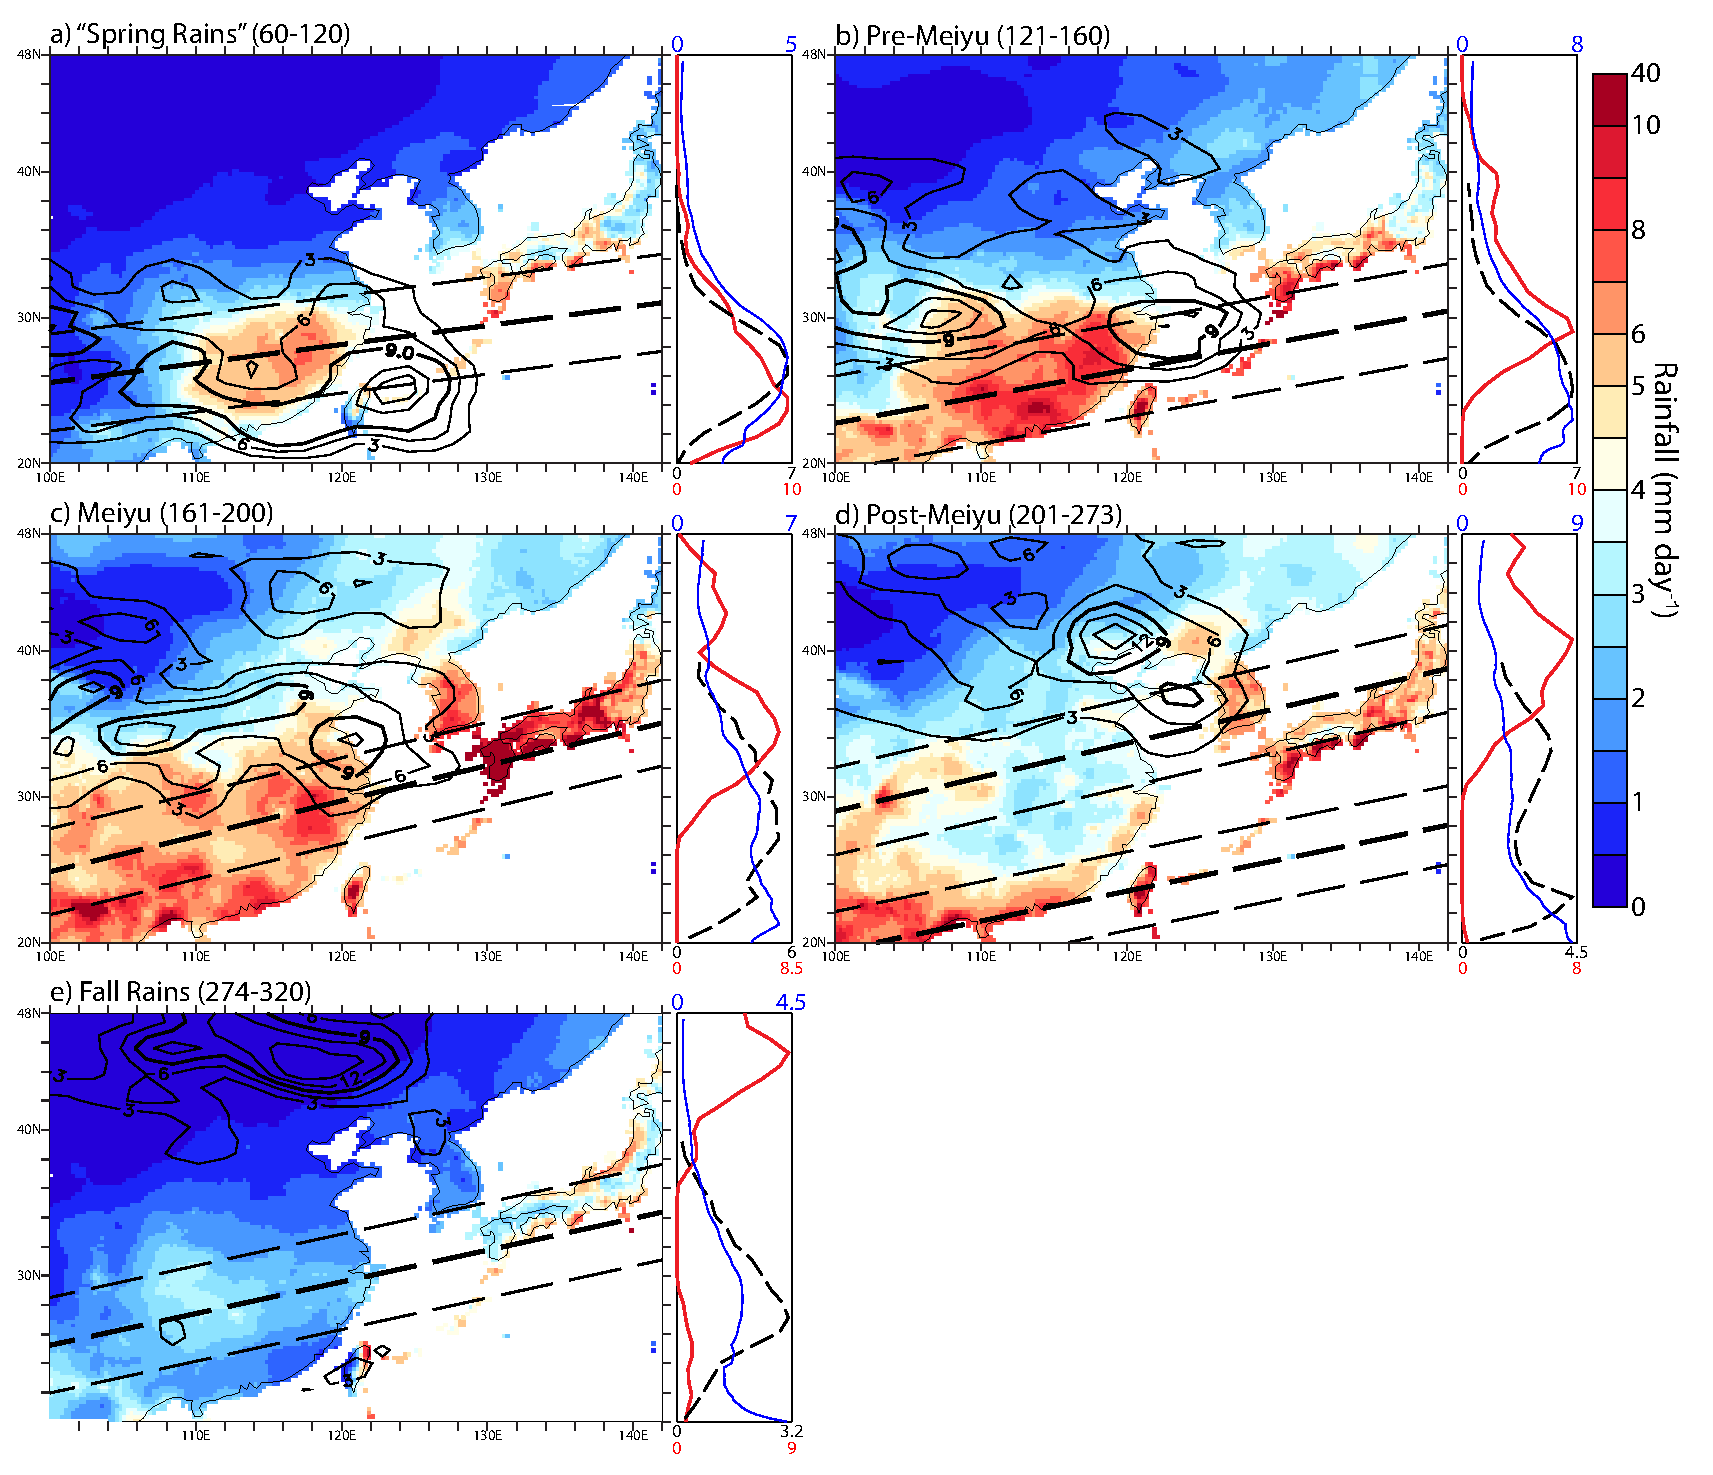
\includegraphics[width=36pc]{Figures/climo}
\caption{a-e: climatology of East Asian rainfall stages, including rainfall (colors), jet frequency (contours; units of probability to the $10^{-4}$) and most common front position during that stage.}
\end{figure}

%%% Changes in Meiyu and rainfall behavior between 1951-1979 and 1980-2007
\begin{figure}[htbp]
\begin{center}
\includegraphics[width=36pc]{Figures/changes}
\caption{a) 15-day running mean of the change in rainfall between 1951-1979 and 1980-07, with 95\%/99\% confidence level marked by single/double cross-hatches. b) 15-day running mean of the change in Meiyu front frequency between 1951-1979 and 1980-07, with two-degree smoothing in latitude and confidence levels marked as in a). In both cases, significance is calculated by bootstrapping over a 15-day running window; for Meiyu frequency, a two-degree latitude window is also used (see Appendix for further description). Time periods are marked as in Figure 1.}
\label{changes}
\end{center}
\end{figure}

%2D spatial distribution of change showing a) full year b) Pre-Meiyu and c) Post-Meiyu
\begin{figure}
\noindent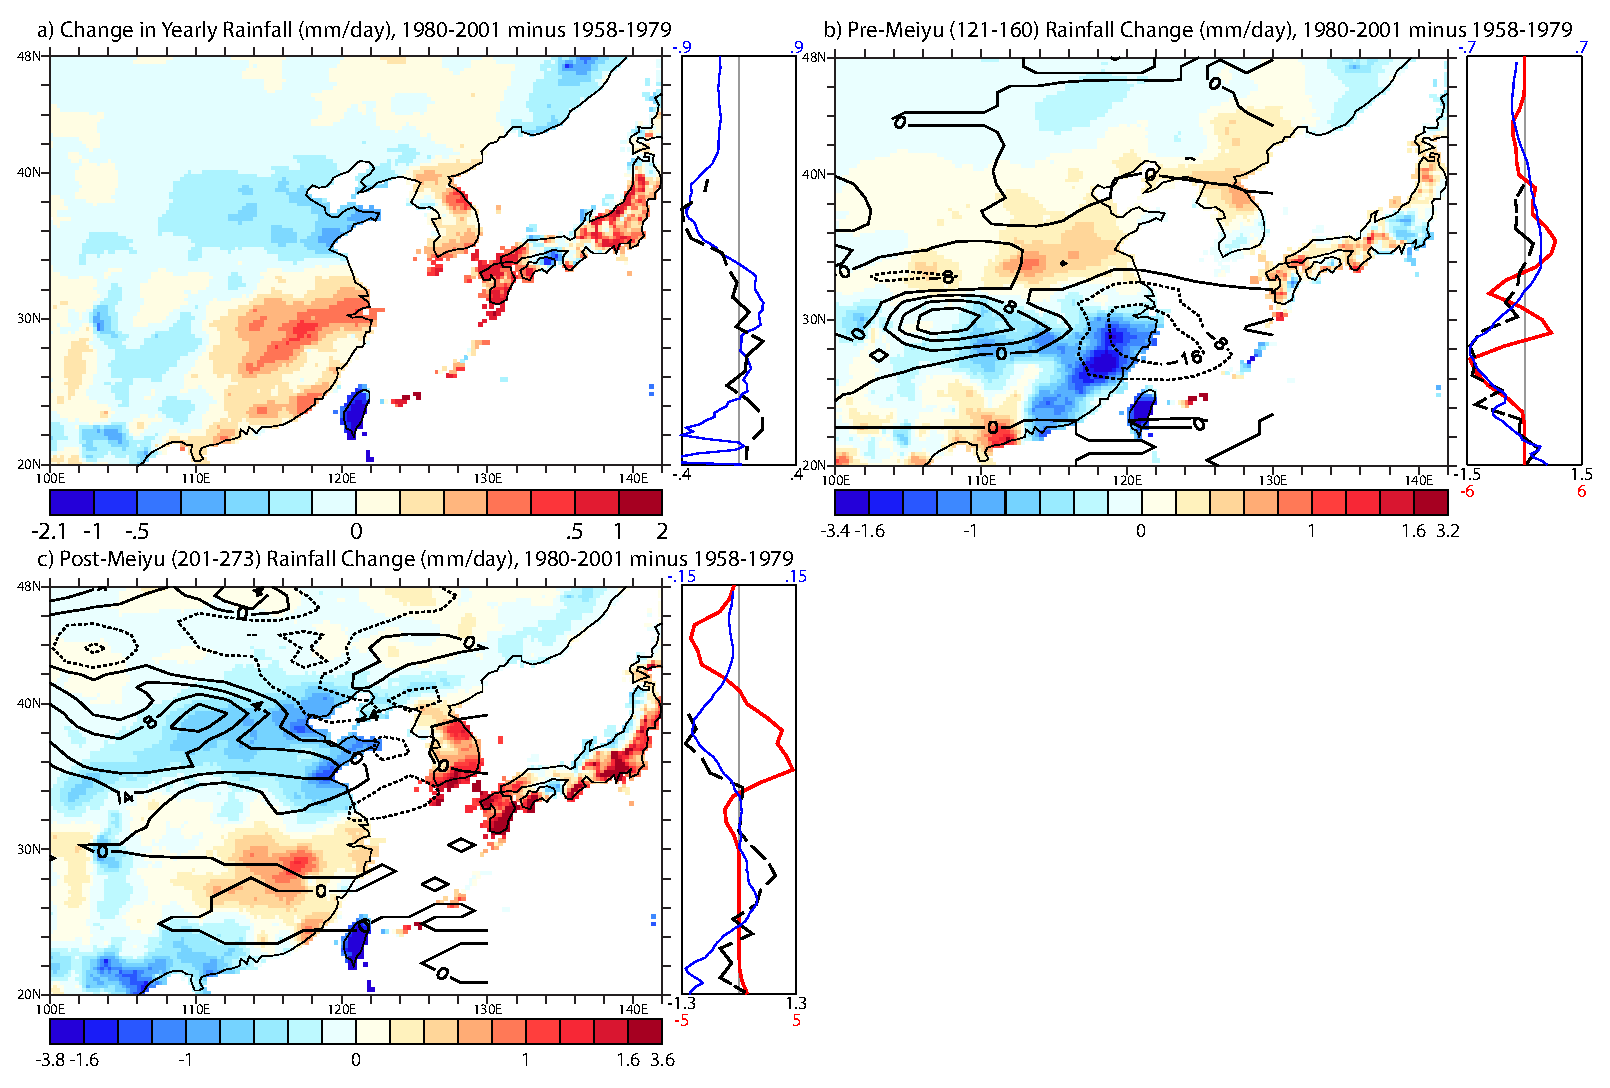
\includegraphics[width=36pc]{Figures/changes_2d}
\caption{a) The ``South Flood-North Drought" pattern of all-year rainfall change; b) Rainfall changes during the Pre-Meiyu (days 121-160) with contours of jet density change overlain; c) Same as c, but for the Post-Meiyu (days 201-273).}
\label{changes_2d}
\end{figure}

%%% Changes in jet mean between 1951-1979 and 1980-2007 + scatter plots of jet and front monthly anomalies.
\begin{figure}[htbp]
\begin{center}
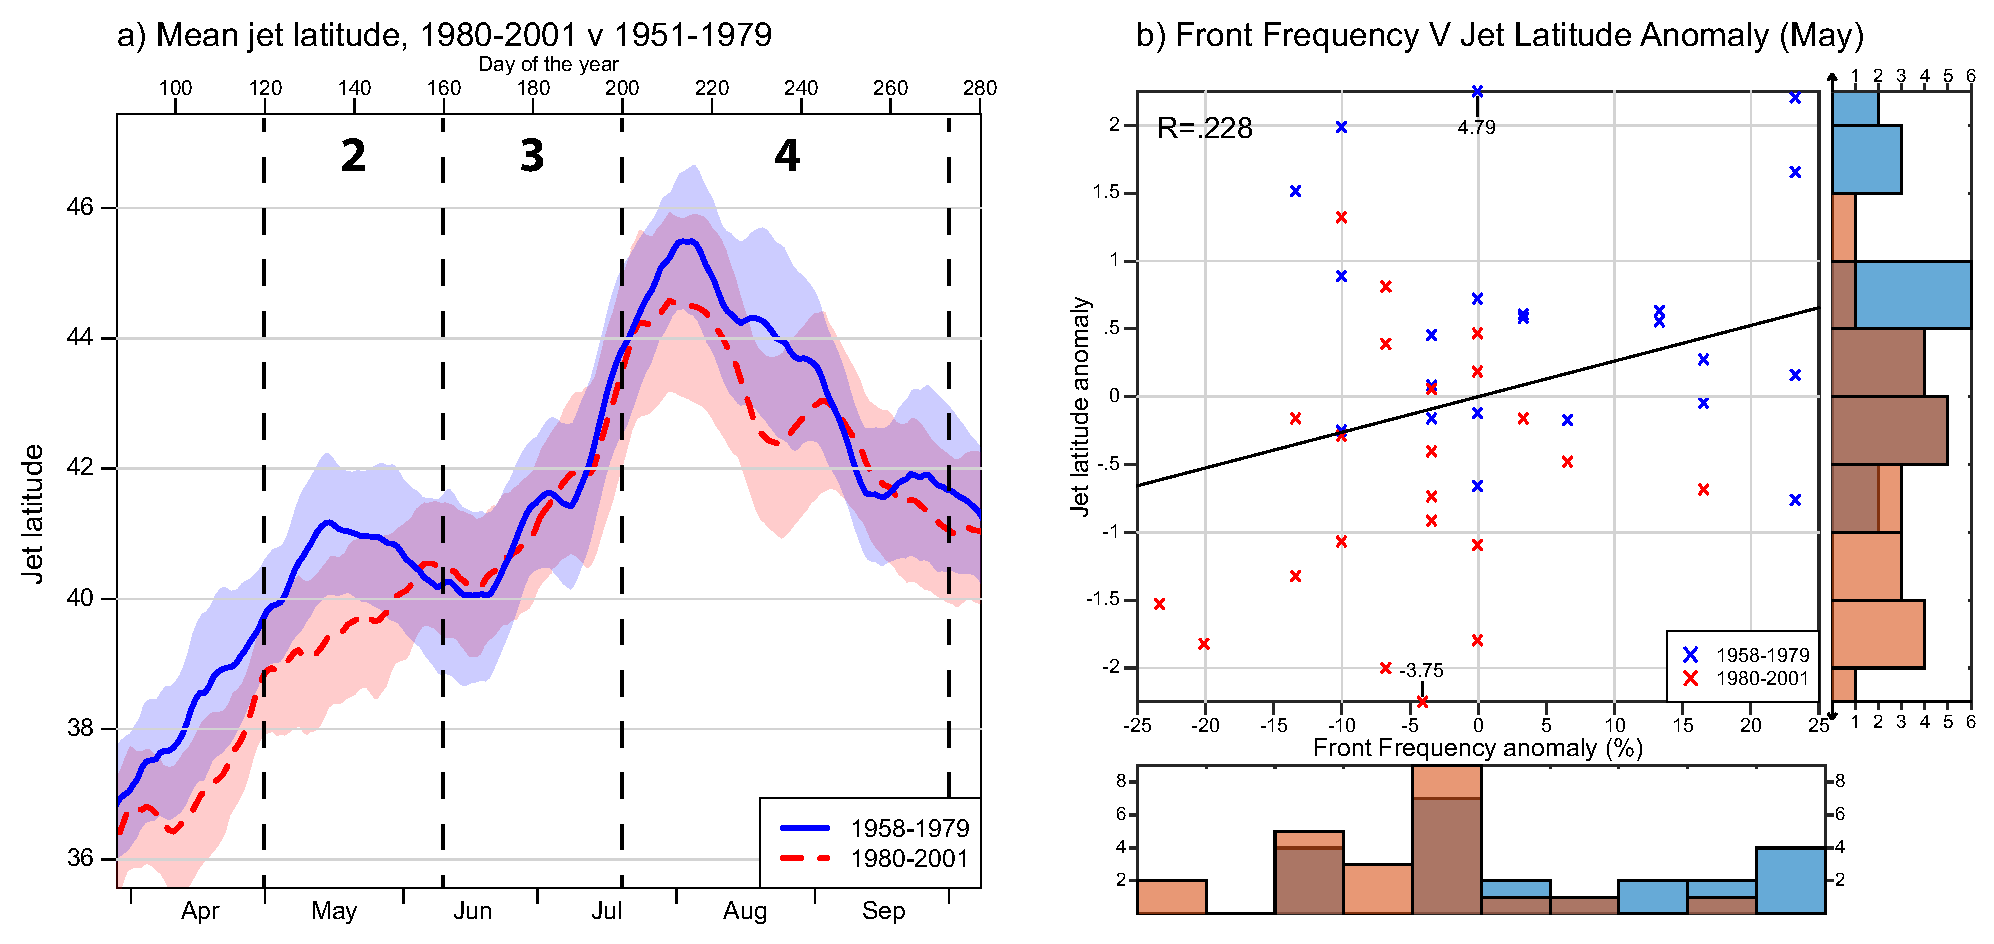
\includegraphics[width=42pc]{Figures/jet}
\caption{a) 7-day running mean latitude of the westerly jet in the region 90-130$^\circ$E for the 1958-1979 (blue, solid) and 1980-2001 (red, dashed). Bootstrapped 95\% confidence intervals are shaded. Time periods: 2 - Pre-Meiyu; 3 - Meiyu; 4 - Post-Meiyu; b) Plot of monthly anomalies in frontal frequency versus monthly anomalies in jet latitude during days 121-150 (May) for 1958-1979 (blue) versus 1980-2001 (red), with anomalies also shown in histogram form.}
\label{jet_seasonal}
\end{center}
\end{figure}
%potential change to implement: add location of Tibetan Plateau to plot.

\end{document}

%% ------------------------------------------------------------------------ %%
%
%  SECTION HEADS
%
%% ------------------------------------------------------------------------ %%

% Capitalize the first letter of each word (except for
% prepositions, conjunctions, and articles that are
% three or fewer letters).

% AGU follows standard outline style; therefore, there cannot be a section 1 without
% a section 2, or a section 2.3.1 without a section 2.3.2.
% Please make sure your section numbers are balanced.
% ---------------
% Level 1 head
%
% Use the \section{} command to identify level 1 heads;
% type the appropriate head wording between the curly
% brackets, as shown below.
%
%An example:
%\section{Level 1 Head: Introduction}
%
% ---------------
% Level 2 head
%
% Use the \subsection{} command to identify level 2 heads.
%An example:
%\subsection{Level 2 Head}
%
% ---------------
% Level 3 head
%
% Use the \subsubsection{} command to identify level 3 heads
%An example:
%\subsubsection{Level 3 Head}
%
%---------------
% Level 4 head
%
% Use the \subsubsubsection{} command to identify level 3 heads
% An example:
%\subsubsubsection{Level 4 Head} An example.
%
%% ------------------------------------------------------------------------ %%
%
%  IN-TEXT LISTS
%
%% ------------------------------------------------------------------------ %%
%
% Do not use bulleted lists; enumerated lists are okay.
% \begin{enumerate}
% \item
% \item
% \item
% \end{enumerate}
%



%% ------------------------------------------------------------------------ %%
%
%  SIDEWAYS FIGURE AND TABLE EXAMPLES
%
%% ------------------------------------------------------------------------ %%
%
% For tables and figures, add \usepackage{rotating} to the paper and add the rotating.sty file to the folder.
% AGU prefers the use of {sidewaystable} over {landscapetable} as it causes fewer problems.
%
% \begin{sidewaysfigure}
% \includegraphics[width=20pc]{samplefigure.eps}
% \caption{caption here}
% \label{label_here}
% \end{sidewaysfigure}
%
%
%
% \begin{sidewaystable}
% \caption{}
% \begin{tabular}
% Table layout here.
% \end{tabular}
% \end{sidewaystable}
%
%

